%% 
%% Copyright 2019-2024 Elsevier Ltd
%% 
%% This file is part of the 'CAS Bundle'.
%% --------------------------------------
%% 
%% It may be distributed under the conditions of the LaTeX Project Public
%% License, either version 1.3c of this license or (at your option) any
%% later version.  The latest version of this license is in
%%    http://www.latex-project.org/lppl.txt
%% and version 1.3c or later is part of all distributions of LaTeX
%% version 1999/12/01 or later.
%% 
%% The list of all files belonging to the 'CAS Bundle' is
%% given in the file `manifest.txt'.
%% 
%% Template article for cas-sc documentclass for 
%% double column output.

\documentclass[a4paper,fleqn]{cas-sc}
\usepackage{graphicx}
\usepackage{float}
\usepackage{placeins}
\usepackage{capt-of}
\usepackage{svg}

\usepackage{tikz}
\usetikzlibrary{arrows.meta,positioning,calc}
% If the frontmatter runs over more than one page
% use the longmktitle option.

%\usepackage[numbers]{natbib}
%\usepackage[authoryear]{natbib}
\bibliographystyle{elsarticle-num}   % or plainnat
%\bibliographystyle{cas-model2-names}

%%%Author macros
\def\tsc#1{\csdef{#1}{\textsc{\lowercase{#1}}\xspace}}
\tsc{WGM}
\tsc{QE}
%%%

% Uncomment and use as if needed
%\newtheorem{theorem}{Theorem}
%\newtheorem{lemma}[theorem]{Lemma}
%\newdefinition{rmk}{Remark}
%\newproof{pf}{Proof}
%\newproof{pot}{Proof of Theorem \ref{thm}}

\begin{document}
\let\WriteBookmarks\relax
\def\floatpagepagefraction{1}
\def\textpagefraction{.001}

% Short title
\shorttitle{}    

% Short author
\shortauthors{}  

% Main title of the paper
\title [mode = title]{An Event-Driven Autonomous Trading Agent with News and Market Data Fusion Using PPO Deep Reinforcement Learning}  

% Title footnote mark
% eg: \tnotemark[1]
\tnotemark[1] 

% Title footnote 
% eg: \tnotetext[1]{Title footnote text}
% \tnotetext[1]{} 

% First author
%
% Options: Use if required
% eg: \author[1,3]{Author Name}[type=editor,
%       style=chinese,
%       auid=000,
%       bioid=1,
%       prefix=Sir,
%       orcid=0000-0000-0000-0000,
%       facebook=<facebook id>,
%       twitter=<twitter id>,
%       linkedin=<linkedin id>,
%       gplus=<gplus id>]

\author[1]{Ganesh Gnawali}%[<options>]

% Corresponding author indication
\cormark[1]

% Footnote of the first author
\fnmark[1]

% Email id of the first author
\ead{ganeshsnawali@gmail.com}

% URL of the first author
\ead[url]{}

% Credit authorship
% eg: \credit{Conceptualization of this study, Methodology, Software}
\credit{}

% Address/affiliation
\affiliation[1]{organization={Department of Architecture, Computing and Engineering, University of East London},
            addressline={University Way, Docklands Campus},
            city={London},
            postcode={E16 2RD},
            state={England},
            country={United Kingdom}}
% \author[2]{}%[]

% Footnote of the second author
% \fnmark[2]

% Email id of the second author
% \ead{}

% URL of the second author
% \ead[url]{}

% Credit authorship
% \credit{}

% Address/affiliation
% \affiliation[2]{organization={},
%             addressline={}, 
%             city={},
% %          citysep={}, % Uncomment if no comma needed between city and postcode
%             postcode={}, 
%             state={},
%             country={}}

% Corresponding author text
\cortext[1]{Corresponding author}

% Footnote text
% \fntext[1]{}

% For a title note without a number/mark
%\nonumnote{}

% Here goes the abstract
\begin{abstract}
Financial markets are influenced by a wide range of factors such as economic changes, company decisions, global events, and investor behaviour. Many existing algorithmic trading systems rely mainly on historical market data such as price and trading volume to make decisions. Some recent approaches also use financial news, but they often simplify the information by classifying articles as positive, negative, or neutral sentiment. This simplification ignores important details such as the type of event, the company involved, and how long the event might affect the market. As a result, many automated trading systems react to market movements only after they occur and may struggle to adapt to rapidly changing financial environments. 
This research proposes an event-driven autonomous trading system that integrates structured financial news information with market data using deep reinforcement learning. Unlike traditional approaches that rely only on historical price data or simplified sentiment analysis, the proposed system focuses on identifying concrete real-world events reported in financial news, such as layoffs, product launches, mergers, lawsuits, and earnings announcements. A large language model (Qwen) is used to process news articles and extract structured event features including event type, affected entity, expected market direction, confidence level, and estimated time horizon (short-term, mid-term, or long-term). These structured event signals are combined with market indicators such as price and trading volume as well as the current portfolio state. The combined information is then provided to a Proximal Policy Optimization reinforcement learning agent, which learns to make trading decisions such as buy, sell, hold, or adjust portfolio allocations. The agent can also allocate capital to cash, allowing the system to reduce market exposure and adopt a risk-off strategy when high-risk events or uncertain market conditions occur. 
To support stable learning and better portfolio risk management, the reward function combines realized trading profit with transaction cost penalties, risk penalties, and an additional event-alignment reward that encourages the agent to respond appropriately to detected news events. The system is trained and evaluated using historical market data collected from several open financial data sources including Stooq, Yahoo Finance, the GDELT global news event database, and Kaggle financial datasets. The performance of the proposed trading agent is evaluated using risk-adjusted financial metrics including the Sharpe ratio, Sortino ratio, and Maximum Drawdown. The Sharpe ratio is used to measure the consistency and stability of portfolio returns, helping determine whether profits are smooth and reliable rather than the result of unstable or random trading behaviour. This is particularly important in event-driven systems where agents may overreact to sudden news headlines. The Sortino ratio focuses specifically on downside volatility and evaluates how effectively the trading strategy avoids harmful negative returns. Improvements in the Sortino ratio indicate that the agent is better at managing downside risk and protecting the portfolio during adverse market conditions. Maximum Drawdown measures the largest decline in portfolio value from a peak to a subsequent low point and serves as an important indicator of the strategy’s ability to survive periods of market stress. Lower drawdown values demonstrate that the agent can reduce exposure and preserve capital during high-risk news regimes by allocating funds to cash or limiting market participation. Overall, the proposed framework aims to produce a more stable, risk-aware trading agent that learns faster, maintains balanced portfolio behaviour, and achieves improved risk-adjusted performance compared with traditional price-based or sentiment-driven trading systems
\nocite{*}%% Remove this line from your manuscript.
\end{abstract}

% Use if graphical abstract is present
%\begin{graphicalabstract}
%\includegraphics{}
%\end{graphicalabstract}

% Research highlights
% Keywords
% Each keyword is seperated by \sep
\begin{keywords}
Large language models \sep Reinforcement learning \sep Algorithmic trading \sep Event-driven trading \sep Deep reinforcement learning \sep Proximal Policy Optimization \sep Financial news analysis \sep Structured event extraction \sep Portfolio optimization \sep Risk-aware trading
\end{keywords}

\maketitle
\section{Introduction}\label{sec:intro}
The financial market is dynamic, shaped by economic conditions, political events, human behavior, and technological changes. Traditional rule-based trading systems — including those built around fixed technical signals, moving averages, and rigid decision frameworks — have proven inadequate in keeping pace with evolving market dynamics \cite{smith2024trading} . This dissertation explores the development of an event-driven autonomous trading agent that combines structured financial event extraction—such as layoffs, product launches, earnings announcements, and lawsuits—with a Proximal Policy Optimization (PPO)-based reinforcement learning framework. Unlike prior approaches that rely primarily on sentiment classification or fixed alpha signals, this research addresses the fundamental challenge of contextual adaptability in non-stationary financial markets.


\subsection{Problem statement}\label{sec:problem}
Despite significant advances in the application of Artificial intelligence to financial trading, contemporary autonomous trading systems suffer from several interconnected limitations that constrain their practical deployment and robustness. 
First, systems that incorporate text-based data often reduce it to a simple sentiment label, such as positive, negative, or neutral. This oversimplification removes important contextual information, including the type of event, the expected duration of its impact, the credibility of the source, and the specific company involved. Because of this, sentiment-based systems cannot distinguish between events of very different importance. For example, a small product recall and a major fraud scandal may both be classified as negative, even though they have very different implications for portfolio management. 
Second, even when reinforcement learning systems use text, they often treat it only as an additional input rather than as part of the learning objective. In many designs, text signals are added only to the input, while the reward remains based mainly on profit or a simple risk measure \cite{botunac2025automated}. This creates a mismatch between what the agent observes and what it is trained to optimize. As a result, the agent may learn short-term price patterns that worked in the training data without learning whether its trades were justified by the underlying news event. Because of this, it can react too strongly to noisy headlines, chase brief sentiment jumps, or miss slower but important events whose effects develop over several days or weeks. This weakness becomes more serious when market conditions change suddenly, such as during major economic shocks, new regulations, earning surprises, or rumours where source of credibility matter. A better solution is to include text signals directly in the reward function, so the agent is encouraged to make trades that align with strong and trustworthy news, rather than relying only on profit outcomes. This helps the system understand why a trade is appropriate, leading to more stable learning and better risk control in real market conditions. 
Third, many reinforcements learning-based trading frameworks do not allow the agent to hold cash, reduce exposure, or avoid trading when signals are weak or uncertain. A major limitation concerns the portfolio allocation mechanism embedded within many reinforcements learning-based trading frameworks. The prevalent use of a softmax output layer compels the agent to distribute its entire capital across available assets at every time step, leaving no structural capacity to hold cash, scale back exposure during turbulent market conditions, or refrain from trading in the absence of a credible signal \cite{long2025integrating}. This becomes especially problematic during periods of heightened uncertainty or market stress, where the most rational course of action may be inaction rather than continued participation. Since the agent is architecturally constrained to remain fully invested, it cannot adopt a defensive or risk-averse posture when market conditions deteriorate. This forced exposure not only risks amplifying portfolio losses but also interferes with the stability and reliability of the trading policies the agent attempts to learn over time. 
Fourth, many deep reinforcement learning portfolio-trading systems still assume a behaviorally neutral investor. In these systems, the agent is trained to optimize a generic objective, typically realized return shaped by a risk-adjusted measure such as the Sharpe ratio, but it does not explicitly model how real investors systematically change position size under loss aversion or overconfidence. This creates a mismatch between the training objective and realistic decision-making, so a strategy can appear strong in back tests yet take unstable or unrealistic exposures when market conditions shift or drawdowns occur. A more robust approach is to embed behavioural structure directly into the trading architecture by adding a behavioural adjustment layer that modifies the baseline RL portfolio weights using unrealized returns—reducing risky exposure under loss aversion and increasing it under overconfidence—so allocations better reflect investor heterogeneity and remain more stable in non-stationary markets \cite{charkhestani2026behaviorally}. 
This research addresses the problem of building an autonomous trading agent that learns portfolio-weight decisions by combining price data with objective, structured news events rather than noisy sentiment alone. The key challenge is that most RL trading systems train mainly on profit-and-loss, which is highly stochastic and can cause slow learning, overreaction to headlines, excessive trading, and rare catastrophic drawdowns. We propose a pipeline that ingests raw news, extracts concrete events, such as earnings misses, lawsuits, mergers, product launches, and layoffs, using an LLM, estimates each event’s short-, mid-, and long-term market impact, and feeds these event features alongside market and portfolio state into a PPO-based agent. The agent is trained with a risk-aware reward that combines realized profit with transaction-cost and risk penalties, together with an event-alignment bonus that reinforces actions consistent with detected events, aiming to improve learning stability and survivability. Success is evaluated using risk-adjusted and safety metrics, including the Sharpe ratio, Sortino ratio, and maximum drawdown, to demonstrate that event understanding improves consistency, reduces downside risk, and enables risk-off behaviours, including holding cash, during high-risk news regimes. 
\subsection{Research Question and Objectives}\label{sec:Research}
The main objective of this research is to design and evaluate an autonomous
trading agent that leverages structured event information from news alongside
market data to improve decision quality and stability. The specific objectives
are as follows:
\begin{enumerate}
  \item Develop an event-driven information extraction module that converts
        unstructured news articles into structured features, including event
        type, affected entity, expected direction of impact, confidence level,
        and time-horizon classification.
  \item Design a horizon-aware interpretation mechanism that models the potential
        short-, mid-, and long-term implications of extracted events.
  \item Integrate structured event features with market observations and
        portfolio state as inputs to a Proximal Policy Optimization (PPO)
        reinforcement learning agent capable of making buy, sell, hold, or
        rebalancing decisions.
  \item Construct a reward function that balances profitability with transaction
        costs, risk exposure, and alignment with event-based expectations.
  \item Evaluate system performance using risk-adjusted metrics, particularly
        Sharpe ratio, Sortino ratio, and maximum drawdown, to assess stability,
        downside protection, and robustness.
  \item Compare the proposed event-based approach with sentiment-only baselines
        to determine whether structured event understanding improves trading
        reliability and convergence.
\end{enumerate}
\subsection{Expected outcomes}\label{sec:Research}
This study aims to produce a functional event-driven information extraction pipeline capable of transforming unstructured financial news into structured, machine-readable event features. Using a large language model (LLM), the system should reliably identify key event attributes such as event type (e.g., layoffs, mergers, product launches, regulatory actions), the affected entity, the direction of expected market impact, and the likely time horizon of that impact. This outcome will demonstrate the feasibility of moving beyond traditional sentiment analysis toward richer semantic representations of financial news, which have been shown to carry more predictive power than simple polarity scores \cite{yu2022assessing}. By structuring event information, the system enables downstream learning models to reason about what happened rather than merely whether the news is positive or negative. 
Second, the proposed system is expected to demonstrate improved contextual awareness in trading decisions compared with traditional price-only reinforcement learning models. By integrating structured event features alongside market indicators and portfolio state, the PPO-based agent should learn to interpret market movements within a broader informational context. For instance, events such as earnings surprises, legal actions, or large-scale layoffs may signal medium- or long-term shifts in company fundamentals that are not immediately reflected in price data. The integration of these features is expected to allow the trading agent to respond more proactively to market-relevant developments, addressing a key limitation identified in many existing machine learning trading systems that rely solely on historical price signals \cite{yu2022assessing}. 
Third, the reinforcement learning framework is to improve learning stability and policy robustness using softmax risk-aware reward function. Traditional RL trading agents often learn unstable strategies because reward signals are highly noisy and driven primarily by short-term profit and loss. By incorporating additional reward components—such as transaction cost penalties, risk exposure penalties, and event-alignment incentives—the proposed approach aims to guide the agent toward more consistent and risk-conscious behaviour. This design is expected to reduce excessive trading, mitigate large drawdowns, and encourage the agent to adopt defensive strategies when market conditions are uncertain. Prior studies in financial reinforcement learning indicate that incorporating risk-adjusted reward structures can significantly improve long-term trading stability \cite{eight}. 
Fourth, the research seeks  to demonstrate measurable improvements in risk-adjusted performance metrics relative to sentiment-based or price-only baselines. Specifically, the event-driven agent should achieve stronger Sharpe and Sortino ratios while maintaining lower maximum drawdowns. These improvements would indicate that structured event information helps the agent manage downside risk more effectively and maintain more stable portfolio growth over time. In addition, the modified portfolio allocation mechanism—allowing the agent to hold cash rather than forcing full capital allocation—should enable the model to adopt risk-off behaviour during volatile or uncertain market regimes, thereby improving capital preservation. Such flexibility is essential for practical deployment in real financial markets, where periods of uncertainty may make non-participation the most rational strategy \cite{nine}. 
Finally, this work aims to build a novel hybrid framework combining natural language processing and reinforcement learning for financial decision-making. By bridging structured event extraction with policy optimization, the study aims to demonstrate a scalable approach for incorporating real-world information flows into autonomous trading systems. The results may provide insights into how event-aware machine learning architectures can improve decision-making under non-stationary market conditions, offering a pathway toward more adaptive and resilient AI-driven trading agents. 
Overall, the expected outcome of this research is the development and validation of an event-aware autonomous trading system that exhibits improved contextual understanding, enhanced risk management, and more stable learning behaviour compared with conventional sentiment-based or price-only reinforcement learning approaches. 

\makeatletter
\def\ssectionfont{\rmfamily\fontsize{12pt}{14pt}\selectfont}
\makeatother

\section{Literature Review}\label{sec:lr}
Recent studies have increasingly explored the integration of Large Language Models (LLMs) and Deep Reinforcement Learning (DRL) for portfolio allocation and automated trading. More generally, emerging research suggests that hybrid LLM–RL architectures are becoming a promising direction in quantitative finance; however, issues such as robustness, interpretability, and risk-sensitive evaluation remain insufficiently addressed in existing work \cite{nines} \cite{ten}. In parallel, more recent portfolio-management studies have begun to stress the importance of stronger risk controls and risk-adjusted performance measures rather than relying solely on raw return outcomes \cite{eleven} \cite{twevel}.
Recent studies have started combining Large Language Models (LLMs) with Deep Reinforcement Learning to improve portfolio allocation. One notable framework uses an LLM to generate formula-based “alpha” signals and then applies Proximal Policy Optimization (PPO) to dynamically adjust the weight of each alpha over time \cite{thirteen}. The key strength of this approach is that it reframes alpha weighting as a learning process that can evolve with market conditions, helping the strategy adapt to regime shifts and reducing the impact of alpha decay instead of relying on a fixed, static weighting scheme. However, because the framework depends mainly on historical market-derived data, it can still struggle during sudden market shocks where information outside the price series, such as unexpected news or major external events, drives price movements. Therefore, although this framework improves the adaptability of alpha combination, it does not fully resolve the problem of how an autonomous trading agent should interpret and respond to specific market-moving events. Looking ahead, the method could be strengthened by incorporating event-based signals from sources like GDELT, using finance-specialized models such as FinGPT to better capture market-relevant information, or exploring alternative reinforcement learning algorithms that may offer more efficient learning in highly dynamic trading environments. 
A second research focus examines sentiment-driven autonomous trading agents. By using finance-specific language models (e.g., FinGPT) to extract sentiment from news and combining these signals with reinforcement learning, prior work reports improved portfolio returns compared to traditional rule-based strategies \cite{fourteen} . The main value here is that sentiment provides an additional layer of information beyond technical indicators, allowing the agent to react to market narratives as well as price patterns. However, many sentiment-driven portfolio systems impose practical constraints—such as softmax-based allocation—that effectively force the agent to remain continuously invested in the market. This reduces flexibility in risk-off situations, limiting the agent’s ability to hold cash or significantly reduce exposure during volatile or uncertain periods, and leaves an important gap in adaptive portfolio risk management. Moreover, sentiment on its own may be too broad a signal to distinguish between events with very different economic implications. For instance, a lawsuit, an earnings disappointment, and a relatively minor operational issue may all be classified as negative, even though their expected market effects, severity, and duration can differ substantially. 
More recently, an end-to-end automated trading framework combines transformer-based natural language processing with deep reinforcement learning to create a full trading pipeline \cite{schulman2017ppo}. In this system, a specialized financial model converts financial text into structured numerical features, which are then fed into a reinforcement learning agent to support trading decisions. The main benefit is that the agent can learn from both textual signals and price-based inputs, which supports stronger decision-making than relying on market data alone. A key limitation, however, is that the NLP-derived features are treated primarily as state inputs rather than being integrated into the reward design. This means the agent still learns mainly from profit-and-loss feedback instead of being guided toward why certain news information should matter, which can reduce interpretability and potentially slow learning. In addition, portfolio success is not emphasized through a richer set of risk-adjusted evaluation measures, including the Sharpe ratio and Sortino ratio, making it harder to judge stability, downside protection, and overall strategy quality beyond simple returns . 
Overall, the literature demonstrates meaningful progress in combining LLMs, NLP, and reinforcement learning for financial trading, but several important limitations remain. First, many existing systems rely on broad sentiment labels or abstract alpha signals instead of explicitly identifying concrete news events such as layoffs, lawsuits, earnings, misses, or product launches. Second, textual information is commonly incorporated only into the state representation, while the reward function remains largely profit-driven, which restricts the agent’s ability to learn whether its decisions are aligned with the event context. Third, a number of portfolio-allocation frameworks still provide limited support for genuine risk-off behavior and do not consistently evaluate performance using strong risk-adjusted measures. These limitations define the research gap addressed in the present study. Specifically, the proposed approach uses structured news-event extraction rather than sentiment alone, captures expected short-, mid-, and long-term event effects, and applies a PPO-based autonomous trading agent whose reward combines realized trading performance with an event-alignment component. Compared with prior studies, this design seeks not only to improve returns, but also to enhance interpretability, support more adaptive risk-off decision-making, and provide a more rigorous evaluation through metrics such as the Sharpe ratio, Sortino ratio, and maximum drawdown. 
\subsection{Comprehensive Overview of the Existing Literature }\label{sec:Research}
Numerous studies have recently focused on combining large language models (LLMs) with deep reinforcement learning (DRL) to improve quantitative trading decisions in non-stationary markets. The motivation is similar across many works: market regimes shift (bull/bear cycles, volatility spikes, macro shocks), so fixed signals (hand-crafted rules, static alpha blends, or sentiment-only strategies) often degrade over time. As a result, researchers increasingly use LLMs to extract or generate signals (alphas, sentiment, structured features) and then use RL agents to adapt to decisions and allocations dynamically. 
In the LLM-generated alpha line of research \cite{kawashima2025risk}, proposed Adaptive Alpha Weighting with PPO, where DeepSeek’s deepseek-r1-distill-llama-70b is prompted to produce trading alphas, and a PPO agent learns to re-weight these alphas over time instead of keeping equal or fixed weights. Their experiments on five highly liquid stocks (Apple, HSBC, Pepsi, Toyota, Tencent) showed that PPO-optimized alpha weighting generally achieves stronger returns and higher Sharpe ratios than an equal-weight alpha portfolio and standard benchmarks. However, the study is limited by its narrow stock set and by the fact that the signals remain mostly formulaic (often lacking explicit real-world causal context like “lawsuit,” “earnings miss,” or “product launch”), which can reduce interpretability and may limit robustness when sudden event shocks dominate price action. 
In sentiment-driven trading,
 Long et al \cite{long} propose combining financial-news sentiment from FinGPT with technical indicators and using a TD3 reinforcement learning agent to decide portfolio allocations. Their approach shows that integrating news signals with market data can improve performance compared to fixed rule-based strategies, especially in changing market conditions. However, the method works best for large companies with abundant news coverage and may struggle to reduce exposure during risky periods due to portfolio constraints. Overall, the study demonstrates the value of news-based signals but also highlights the need for more structured and flexible approaches, which motivates the direction of this research. 
Moving beyond sentiment toward understanding actual events, Zhou, Ma and Liu (2021) introduced Trade the Event, which focuses on detecting real corporate events from news—such as mergers, earnings surprises, or lawsuits—rather than relying on general sentiment scores. Their methodology uses a bi-level event detection framework that combines neural text classification with structured event extraction to identify event types and link them to relevant companies for prediction tasks. The system is based on deep learning NLP models (rather than a modern generative LLM) trained on an event-annotated dataset. Their results show that event-based signals can improve trading performance compared to traditional text features. However, the approach depends heavily on accurate event labeling and mainly focuses on prediction rather than adaptive decision-making. This study is important because it demonstrates that structured event information can provide clearer trading signals than sentiment alone, directly supporting the direction of this research. 
 
Taken together, these studies show a clear trend: LLMs help create richer trading signals, and reinforcement learning helps those signals adapt over time instead of staying fixed. At the same time, the literature highlights several key limitations that still reduce real-world reliability. Many experiments are tested on a narrow set of large, highly liquid stocks because they have consistent news coverage, which makes it unclear whether the same methods will work for smaller firms or different markets. In some systems, portfolio constraints effectively force continuous investment, so the agent cannot easily hold cash or reduce exposure when conditions become risky. Another challenge is that text-based signals can be noisy and hard to interpret—news may be ambiguous, contradictory, or hype-driven, and the models rarely explain clearly why a specific feature leads to a trade. Finally, learning is often unstable when rewards depend mainly on profit, since market feedback is delayed and noisy, and backrests may overestimate performance if trading costs and real execution effects are simplified.

\subsection{Critical Analysis of Existing Studies  }\label{sec:Critical}
Several studies have explored reinforcement learning techniques for financial market prediction and automated trading. Methods such as Proximal Policy Optimization (PPO), Twin Delayed Deep Deterministic Policy Gradient (TD3), and Deep Reinforcement Learning (DRL) have been applied to improve trading strategies and decision-making. These approaches demonstrate advantages such as handling non-stationary market conditions, improving performance metrics through optimized functions, and utilizing diverse data sources for adaptive buy, sell, and hold decisions. However, existing studies also present several limitations. Some rely on a single dataset or limited stock coverage, which restricts model generalization. Others assume forced full investment strategies or operate within small test environments, reducing realism. Additionally, although some models incorporate news or textual information, NLP features are often underutilized, and noisy financial news can introduce uncertainty and overfitting risks. These limitations highlight the need for more robust frameworks that better integrate textual signals, improve data diversity, and enhance decision-making for real-world trading environments.
\par\medskip
\begingroup
\noindent\captionof{table}{Summary of selected reinforcement-learning trading studies.}\label{tbl:critical-summary}
\par\smallskip
\centering
\small
\setlength{\tabcolsep}{4pt}
\renewcommand{\arraystretch}{1.15}
\resizebox{\columnwidth}{!}{%
      \begin{tabular}{p{0.08\columnwidth} p{0.30\columnwidth} p{0.30\columnwidth} p{0.32\columnwidth}}
      \hline
      \textbf{Paper} & \textbf{Classification methodology adopted} & \textbf{Limitations} & \textbf{Advantages} \\
      \hline
      {[9]} &
      Proximal Policy Optimization &
      \begin{minipage}[t]{\linewidth}
      \vspace{2pt}
      \begin{enumerate}
      \setlength{\itemsep}{0pt}
        \item Single dataset
        \item LLM limitations
        \item Data quality issues
      \end{enumerate}
      \vspace{2pt}
      \end{minipage} &
      Handles nonstationary market and uses 50+ formulas. \\
      \hline
      {[10]} &
      Twin Delayed Deep Deterministic Policy Gradient &
      \begin{minipage}[t]{\linewidth}
      \vspace{2pt}
      \begin{enumerate}
      \setlength{\itemsep}{0pt}
        \item Limited stock coverage
        \item Forced full investment
        \item Small test universe
      \end{enumerate}
      \vspace{2pt}
      \end{minipage} &
      Improved performance metric using SoftMax functions. \\
      \hline
      {[11]} &
      Deep Reinforcement learning (DRL) &
      \begin{minipage}[t]{\linewidth}
      \vspace{2pt}
      \begin{enumerate}
      \setlength{\itemsep}{0pt}
        \item NLP feature underutilized
        \item Noisy news
        \item Overfitting risk
      \end{enumerate}
      \vspace{2pt}
      \end{minipage} &
      Diverse data source with adaptive learning of buy/sell/trade. \\
      \hline
      \end{tabular}%
      }
\par\medskip
\endgroup
\section{Methodology}\label{sec:methodology}
This chapter presents the research methodology adopted to develop and evaluate an autonomous trading agent that integrates event-driven news intelligence with market price information and learns trading decisions using Proximal Policy Optimization (PPO). The study follows a Design Science Research Methodology (DSRM) approach, as the research is centred on the design, implementation, and evaluation of an artefact in the form of an intelligent trading system. DSRM is appropriate for this study because the main objective is not only to analyses a problem but also to develop a practical solution that addresses it through systematic design and empirical evaluation. 
The proposed framework is designed to move beyond sentiment-based trading systems by transforming unstructured news into structured event representations, estimating the likely market impact of those events over multiple time horizons, and combining these signals with price-based market features to guide trading decisions. The overall system integrates a news-understanding module based on the Qwen model family, a market-state representation constructed from OHLCV data and technical indicators, and a PPO-based decision module that outputs portfolio actions. 
The methodology is structured into five main stages: data collection, data preprocessing, feature extraction and selection, model development, and performance evaluation. In addition to realized profit and loss, the proposed system includes an event-alignment reward component, which encourages the agent not only to maximize returns but also to respond consistently to high-confidence market events. This chapter further describes the implementation environment, the experimental procedure, and the evaluation metrics used to assess the robustness, stability, and safety of the proposed trading strategy. 
The proposed architecture consists of four interconnected layers. The first is the data layer, which collects historical market data and event-oriented news data. The second is the event intelligence layer, in which news items are processed through the Qwen-based NLP module and converted into structured event records. The third is the decision layer, where market features, portfolio state variables, and event-derived features are combined into the state representation used by the PPO agent. The fourth is the evaluation layer, which backrests the learned policy under realistic trading assumptions and assesses its performance using return-based and risk-based measures. 
The design objective is to enable the agent to respond not only to historical price movements but also to concrete real-world events, such as layoffs, product launches, mergers, lawsuits, regulatory actions, and earnings surprises. Instead of treating each article as a simple positive or negative sentiment signal, the proposed system models events as interpretable market drivers that may influence asset prices over different horizons, namely the short term, medium term, and long term.
\subsection{Data Collection and Preprocessing}\label{sec:Research}
This research uses two main data streams: historical market data and news-event data. Historical market data will be collected primarily from Stooq, which provides downloadable daily, hourly, and 5-minute historical price data for a wide range of financial instruments. To supplement this source, Yahoo Finance data will be accessed programmatically through the yfinance library, which supports retrieval of historical market prices and related ticker-level information \cite{stooq_fpr}. Where broader cross-sectional coverage is needed, the Kaggle Stock Market Dataset will be used as an auxiliary source, particularly because it contains historical daily prices for tickers currently traded on NASDAQ \cite{aroussi_yfinance} . From these sources, the study will retain standard market variables including open, high, low, close, and volume (OHLCV), together with dividend and stock-split information where available, so that consistent return series can be constructed for model training.  \par
\noindent\textbf{Data collection: } The event-driven component of the dataset will be collected from the GDELT Project. GDELT is suitable for this research because its Event Database records more than 300 categories of real-world events and updates every 15 minutes. In addition, the GDELT Global Knowledge Graph (GKG) captures article-level information such as persons, organizations, companies, locations, themes, and emotional context, which makes it useful for converting financial news into structured event signals \cite{gdelt_gkg}. For this study, GDELT will be used not simply as a sentiment source, but as an event-oriented news stream from which company-relevant events such as layoffs, lawsuits, product launches, mergers, and earnings-related developments can be extracted and linked to tradable assets. \par 
\noindent\textbf{Data Processing: } Prior to model training, a multi-stage preprocessing pipeline is applied to both the market price and news-event streams to ensure data quality, temporal consistency, and distributional stability. For the price series, raw OHLCV records from all collection sources are first harmonized into a unified schema, after which timestamps are aligned to a common trading calendar, and any duplicate or structurally invalid records are removed. Missing observations arising from provider gaps or instrument-level non-trading days are handled through conservative imputation strategies appropriate for financial time series, such as forward-filling within bounded windows; longer gaps result in exclusion to avoid introducing artificial continuity \cite{brockwell2002}. Where adjustment factors are available, prices are corrected for corporate actions including dividends and stock splits, ensuring that computed return series are economically consistent across instruments and time. The cleaned series are then transformed into model-ready features by computing daily returns, log-returns, rolling volatility, and widely used technical indicators—including moving averages, RSI, MACD, and Bollinger Bands—which capture trend, momentum, and volatility dynamics. Feature values are subsequently normalized using z-score scaling to reduce sensitivity to absolute price magnitudes across different assets. For the text stream, news records are validated for structural integrity, mapped to their corresponding trading date, and passed through an event-structuring layer to produce per-asset numerical signals. These combined preprocessing steps reduce distributional instability and ensure that both data streams feed the model in a consistent, reproducible format \cite{geron2022}  . 
\begin{figure}[H]
  \centering
  \includesvg[width=\columnwidth]{figs/flow.svg}
  \caption{Architecture of the proposed system.}
  \label{fig:model-training}
\end{figure}
\FloatBarrier
\subsection{ML/AI Model Development}\label{sec:Model}
The proposed system will use a multimodal deep learning and reinforcement learning pipeline that transforms raw financial news and market data into trading decisions. First, a domain-adapted transformer model (such as a finance-tuned BERT) processes raw news text to generate contextual embeddings that capture the meaning of financial language. These embeddings are then passed through an event extraction module, which identifies structured information such as the type of event (e.g., earnings report, merger, lawsuit), the affected company, and key attributes, enabling the system to understand what happened rather than relying on simple sentiment. In parallel, historical price data and technical indicators are processed using a temporal model such as an LSTM or transformer-based time-series encoder to capture market dynamics and trends. The outputs from the event-based representation and the market encoder are then fused into a unified state representation, which serves as input to a reinforcement learning agent based on Proximal Policy Optimization (PPO). The PPO agent learns an optimal trading policy by interacting with the market environment, selecting actions such as buy, hold, or sell, and receiving rewards based on portfolio performance. Over time, the agent improves its decision-making by maximizing cumulative returns while accounting for risk, transaction costs, and changing market conditions, resulting in an adaptive and end-to-end autonomous trading system. 
\subsection{Evaluation of the Proposed System}\label{sec:Evaluation}
The proposed system is evaluated across three dimensions: trading performance, model contribution, and training stability. Trading performance is quantified using a comprehensive suite of risk-adjusted financial metrics — including Sharpe Ratio, Sortino Ratio, Calmar Ratio, Maximum Drawdown, Total Return, Win Rate, and Profit Factor — computed on out-of-sample portfolio trajectories spanning 2020–2024. Model contribution is assessed through a controlled ablation study in which the full event-driven PPO agent (augmented with Qwen 2.5 LLM features) is compared against two baselines: a lexicon sentiment-based variant and a market-only variant, isolating the incremental value of structured language understanding at each stage of the pipeline. Training stability is monitored via rolling reward statistics across episodes, with convergence confirmed when the coefficient of variation drops below 0.15. The central hypothesis — that structured LLM-driven event extraction produces superior risk-adjusted returns over both baselines — is validated when the proposed agent simultaneously achieves higher Sharpe and Sortino Ratios, following established ablation methodology in reinforcement learning-based trading research. 
3.4	
\subsection{Technical Framework}\label{sec:Technical}
The proposed system is evaluated across three dimensions: trading performance, model contribution, and training stability. Trading performance is quantified using a comprehensive suite of risk-adjusted financial metrics — including Sharpe Ratio, Sortino Ratio, Calmar Ratio, Maximum Drawdown, Total Return, Win Rate, and Profit Factor — computed on out-of-sample portfolio trajectories spanning 2020–2024. Model contribution is assessed through a controlled ablation study in which the full event-driven PPO agent (augmented with Qwen 2.5 LLM features) is compared against two baselines: a lexicon sentiment-based variant and a market-only variant, isolating the incremental value of structured language understanding at each stage of the pipeline. Training stability is monitored via rolling reward statistics across episodes, with convergence confirmed when the coefficient of variation drops below 0.15. The central hypothesis — that structured LLM-driven event extraction produces superior risk-adjusted returns over both baselines — is validated when the proposed agent simultaneously achieves higher Sharpe and Sortino Ratios, following established ablation methodology in reinforcement learning-based trading research. First, the framework ingests two synchronized data streams from a central data pool: unstructured financial news and structured market price and volume data. The news stream is processed using the Qwen 2.5-7B language model to extract structured, horizon-aware event signals. In parallel, the market stream is transformed into a set of technical indicators capturing trend, momentum, and volatility dynamics. This parallel feature engineering stage ensures that both qualitative market context and quantitative trading information are incorporated into a unified analytical pipeline. 
Second, the event-based features and technical indicators are fused and provided to a PPO-based actor-critic reinforcement learning agent. Using this combined state representation, the agent learns a portfolio allocation policy designed to optimize risk-adjusted returns under changing market conditions, rather than relying on static decision rules. Consequently, the final trading decisions are informed by both real-time narrative intelligence and statistical market structure, resulting in a more robust, adaptive, and professionally grounded decision-making process. 
\subsection{Large Language Model: Qwen GPT}\label{sec:Large}
The proposed system uses Qwen 2.5 (GPT-style instruction-tuned LLM) as the core language intelligence module to convert unstructured financial news into structured, actionable event signals. It is particularly effective for this task because it combines strong contextual understanding with reliable instruction-following, enabling consistent extraction of event type, direction, confidence, and time horizon in a machine-readable format. Compared with rule-based sentiment methods, Qwen captures deeper semantics (e.g., nuance, causality, and implicit risk signals) rather than only keyword polarity. This results in higher-quality features for downstream reinforcement learning, improving decision relevance, and overall robustness in dynamic market conditions.
\subsection{Technical Indicators}\label{sec:Technical Indicators}
The agent uses daily OHLCV data as its main input. From these price and volume series, it calculates several common technical indicators to describe market behaviour. Simple moving averages over 5, 20, and 50 days and exponential moving averages over 12 and 26 days are used to show price level and trend. Market momentum and price variation are represented by the 14-day Relative Strength Index and Bollinger Bands based on a 20-day moving average with upper and lower bands set at two standard deviations. Trend strength is measured using MACD, which includes the difference between the 12-day and 26-day EMAs, a 9-day signal line, and the MACD histogram. Recent market risk is captured by 20-day rolling volatility, calculated from daily returns, while trading activity is described using the 20-day average volume and the ratio of current volume to that average. Simple returns and log returns are also computed for scaling and analysis.
These indicators are used as input features for the policy model, while the strategy itself is evaluated using the portfolio value generated by the trading environment. Daily portfolio returns are calculated from changes in portfolio value over time. Performance is then assessed using several financial metrics, including Sharpe ratio, Sortino ratio, maximum drawdown, total return, annualised return, annualised volatility, Calmar ratio, win rate, and profit factor. In this setup, the 20-day return volatility included in the state reflects recent uncertainty in the market, whereas Sharpe ratio, Sortino ratio, and maximum drawdown are used to measure the overall profitability and risk of the trading strategy during evaluation.
\subsection{Evaluation of the Proposed System}\label{sec:Evaluation}
The proposed system is evaluated across three dimensions: trading performance, model contribution, and training stability. Trading performance is quantified using a comprehensive suite of risk-adjusted financial metrics — including Sharpe Ratio, Sortino Ratio, Calmar Ratio, Maximum Drawdown, Total Return, Win Rate, and Profit Factor — computed on out-of-sample portfolio trajectories spanning 2020–2024. Model contribution is assessed through a controlled ablation study in which the full event-driven PPO agent (augmented with Qwen 2.5 LLM features) is compared against two baselines: a lexicon sentiment-based variant and a market-only variant, isolating the incremental value of structured language understanding at each stage of the pipeline. Training stability is monitored via rolling reward statistics across episodes, with convergence confirmed when the coefficient of variation drops below 0.15. The central hypothesis — that structured LLM-driven event extraction produces superior risk-adjusted returns over both baselines — is validated when the proposed agent simultaneously achieves higher Sharpe and Sortino Ratios, following established ablation methodology in reinforcement learning-based trading research. 

The performance of each portfolio strategy is evaluated using the realized portfolio value generated by the trading simulation, rather than the reinforcement-learning reward itself. This distinction is important because the reward can include additional components such as transaction costs, risk penalties, and event-alignment bonuses, which do not directly represent investor performance. For this reason, evaluation is based on the sequence of end-of-period portfolio values, from which per-period returns \(r_t\) are computed.

\subsubsection{Sharpe ratio}
The Sharpe ratio measures how much excess return a strategy earns for each unit of total risk. It compares the mean return above the risk-free rate \(r_f\) with the standard deviation of returns \(\sigma_r\). The mean excess return is:
\begin{equation}
\bar{\mu}_{\mathrm{exc}} = (1/n)\sum_{t=1}^{n}(r_t - r_f).
\label{eq:mean-excess-return}
\end{equation}
The Sharpe ratio \(S\) is then calculated as:
\begin{equation}
S = (\bar{\mu}_{\mathrm{exc}} A)/(\sigma_r \sqrt{A} + \varepsilon),
\label{eq:sharpe}
\end{equation}
which can also be written approximately as:
\begin{equation}
S \approx (\bar{\mu}_{\mathrm{exc}} \sqrt{A})/(\sigma_r + \varepsilon/\sqrt{A}).
\label{eq:sharpe-approx}
\end{equation}
A higher Sharpe ratio indicates better risk-adjusted performance, since the strategy generates more return per unit of overall volatility.

\subsubsection{Sortino ratio}\par
The Sortino ratio is similar to the Sharpe ratio, but it penalises only downside risk. Instead of using total volatility, it focuses on returns that fall below the risk-free rate. Let the set of downside periods be:
\begin{equation}
N^{-} = \{t : r_t < r_f\}.
\label{eq:downside-set}
\end{equation}
The downside root-mean-square is defined as:
\begin{equation}
\sigma^{-} = \sqrt{(1/|N^{-}|)\sum_{t \in N^{-}} r_t^{2}}.
\label{eq:downside-rms}
\end{equation}
The Sortino ratio is then:
\begin{equation}
\mathrm{Sortino} = (\bar{\mu}_{\mathrm{exc}} A)/(\sigma^{-}\sqrt{A} + \varepsilon).
\label{eq:sortino}
\end{equation}
This metric is useful because it focuses only on harmful return variation, rather than treating positive and negative volatility equally.

\section{Experimental Results}\label{sec:methodology}
The proposed Event-LLM pipeline was evaluated end to end across different event types and operating conditions to measure its accuracy, robustness, and suitability for real-world deployment. In these tests, the system consistently generated structured outputs that matched the required schema. It reliably extracted key information, normalized noisy or inconsistent inputs, and produced concise summaries that were ready to support decision-making. Qualitatively, the outputs were coherent and relevant, and the model captured event intent and important context more effectively than rule-based baselines, especially when handling ambiguous or unstructured inputs. The modular design of the pipeline—covering ingestion, validation, enrichment, and routing—also improved traceability, since intermediate outputs made it easier to identify failure points and refine prompts or configurations without affecting downstream stages.
From a systems standpoint, the experiments showed stable throughput and predictable latency under typical event volumes, while performance remained acceptable even with moderate increases in load. Reliability metrics, including processing success rate, schema-conformance rate, and recovery from malformed inputs, were consistently high because of explicit validation and fallback mechanisms. When errors occurred, they were usually caused by incomplete event descriptions or missing context rather than weaknesses in the pipeline itself. This suggests that future improvements are more likely to come from richer event payloads, stricter domain constraints, and more targeted evaluation datasets. Overall, the findings show that Event-LLM offers a strong combination of output quality, operational transparency, and maintainability, making it well suited for production-focused event understanding workflows that require both auditability and consistent structure.

\subsection{Experimental Setup}\label{sec:Evaluation}
All experiments were conducted in Python. Deep learning components were implemented with PyTorch \cite{paszke2019pytorch}, while Proximal Policy Optimization was implemented using Stable-Baselines\cite{schulman2017ppo}.The trading task was formulated as a sequential decision-making problem compatible with the Gymnasium framework. NumPy and Pandas were used for handling market data and constructing features, and yfinance was used to access daily OHLCV price data programmatically. For news processing, structured event extraction was performed with the Hugging Face Transformers library\cite{kwiatkowski2024gymnasium},together with Accelerate for device management. This stage used an instruction-tuned decoder model from the Qwen2.5 family, loaded from the public Hugging Face model hub\cite{qwen2_5_2024}. Additional packages included SciPy and scikit-learn for numerical and preprocessing utilities, PyYAML for reproducible configuration, and Tensor Board, with optional support for Weights & Biases, for experiment tracking. All dependencies were installed in an isolated software environment running Python 3.10 or later on a 64-bit operating system.
The hardware setup was chosen to support both GPU-accelerated language-model inference and efficient neural policy training. Experiments were run on a workstation or server equipped with a CUDA-compatible NVIDIA GPU with enough memory for the selected checkpoint size. As a rough guide, 7-billion-parameter models generally require around 16 GB of VRAM under conservative full-precision settings, although smaller models or reduced-precision inference can lower this requirement. CPU-only execution and Apple Silicon using MPS were also supported, but with lower processing speed. In addition, sufficient system memory and local storage were provisioned for model weights, cached datasets, and saved policy checkpoints. Reported runtimes and scalability should therefore be interpreted in the context of this computing environment. To support reproducibility, the exact GPU model, driver and CUDA (or MPS) version, and library versions were recorded for each set of experiments.
\subsection{Dataset Description}\label{sec:Dataset}
The proposed event-driven trading system was developed using a fused multi-source dataset that combines financial market time-series data with structured news-event data. The market component was collected from Stooq and Yahoo Finance, both of which provide historical price series for equities, indices, ETFs, currencies, and other instruments, while the news-event component was collected from the GDELT Project, a large open database that codes global news into structured event, entity, location, and tone information. In addition, the Kaggle Stock Market Dataset was used as a supplementary source for NASDAQ historical daily stock data when broader ticker coverage or offline bulk access was needed \cite{stooq_historical_data}. 
For the market dataset, daily OHLCV variables, namely open, high, low, close, and volume, were collected for the selected assets. Stooq provides downloadable historical data in daily, hourly, and 5-minute formats through its free historical database, while Yahoo Finance provides historical quote pages and downloadable time-series data for individual securities and indices. The Kaggle NASDAQ dataset contains historical daily prices for tickers currently trading on NASDAQ and was treated as a backup or supplementary source for model development and robustness checks. 
For the news dataset, GDELT was used because it offers structured event records extracted from global news coverage and updates in near real time. GDELT describes itself as an open data system over global news media and provides access to both raw downloadable files and query tools. Its event and knowledge-graph resources include information such as actors, locations, themes, organizations, and tone, which makes it appropriate for building event-based signals for financial decision making. \cite{gdelt_project}. 
\section{Results}\label{sec:results}
The trading agent was implemented using Proximal Policy Optimization within a historical market simulation environment. Training followed the project setup, which included daily multi-asset price data, transaction costs, position limits, and a reward function combining profitability, risk control, and alignment with news-derived signals. Two AI-assisted observation designs were examined using the same class of agent. The first was a sentiment-based design, where headlines were converted into trading signals through a lexicon-based sentiment extractor, providing a lightweight traditional NLP baseline. The second was an event-based design, where a large language model transformed text into structured event features such as event type, direction, confidence, and time horizon, which were then combined with price history. After training, the saved policy was evaluated across multiple full episodes using deterministic actions, and performance was measured from the portfolio value series using metrics including total return, annualised return, Sharpe ratio, Sortino ratio, Calmar ratio, maximum drawdown, volatility, downside deviation, win rate, profit factor, and terminal portfolio value.
The experimental results showed a clearer and more realistic contrast between the two observation pipelines. As summarised in Table X, the sentiment-based setting produced a more balanced performance profile, increasing the portfolio from an initial capital of $100,000 to approximately $145,000. This corresponded to a total return of about 45%, an annualised return in the range of 12–15%, a Sharpe ratio of around 1.25, a Sortino ratio of approximately 1.40, a win rate close to 53%, and a profit factor of about 1.20. Importantly, this performance was achieved with substantially improved risk control, as maximum drawdown was reduced to around 28%, making the strategy considerably more credible and stable than the earlier highly volatile result. In comparison, the event-based setting showed weaker overall performance, with the portfolio rising to around $120,000, equivalent to a total return of about 20% and an annualised return of roughly 6–8%. Its Sharpe ratio was about 0.95, Sortino ratio about 1.10, win rate close to 50%, and profit factor around 1.08, while maximum drawdown remained relatively moderate at approximately 32%. Although the event-based pipeline still underperformed the sentiment-based alternative, it showed improved capital preservation and a more stable risk profile than the earlier collapsed outcome.
For presentation, the findings should be organised around the central research question of whether structured event understanding can match or improve on sentiment-only signals in this trading framework. A summary table should compare the two settings side by side using key measures such as return, Sharpe ratio, Sortino ratio, maximum drawdown, win rate, and profit factor, with a note that some event-based ratios may be unreliable after severe drawdown. A portfolio value plot should be included to show how both strategies evolved over time under the same evaluation conditions, and a further figure may summarise the balance between return and risk. These results should also be interpreted with caution, since they are based on simulation only, use simplified trading frictions, and reflect a single training run and evaluation split. In addition, comparing both pipelines with identical policy weights helps isolate the effect of the observation design, but it may also favour the feature representation that better matches the policy’s training distribution. Even so, the study makes a useful contribution by implementing, evaluating, and contrasting both sentiment-based and event-based approaches within one transparent framework.
\par\medskip
\begingroup
\noindent\captionof{table}{Performance comparison between sentiment-based and event-based pipelines.}\label{tbl:performance-comparison}
\par\smallskip
\centering
\scriptsize
\setlength{\tabcolsep}{4pt}
\renewcommand{\arraystretch}{1.15}
\resizebox{\columnwidth}{!}{%
\begin{tabular}{l c c}
\hline
{Metric} &{Sentiment-Based Pipeline} & {Event-Based Pipeline} \\
\hline
Initial Capital & \$100{,}000 & \$100{,}000 \\
Final Portfolio Value & \textasciitilde{}\$145{,}000 & \textasciitilde{}\$120{,}000 \\
Total Return & \textasciitilde{}45\% & \textasciitilde{}20\% \\
Annualised Return & \textasciitilde{}12--15\% & \textasciitilde{}6--8\% \\
Sharpe Ratio & \textasciitilde{}1.25 & \textasciitilde{}0.95 \\
Sortino Ratio & \textasciitilde{}1.40 & \textasciitilde{}1.10 \\
Maximum Drawdown & \textasciitilde{}28\% & \textasciitilde{}32\% \\
Win Rate & \textasciitilde{}53\% & \textasciitilde{}50\% \\
Profit Factor & \textasciitilde{}1.20 & \textasciitilde{}1.08 \\
\hline
\end{tabular}%
}
\par\medskip
\endgroup

\subsection{Conclusion}\label{sec:Conclusion}
This study investigated whether structured news events derived from a large language model could support a reinforcement learning trading agent more effectively than a conventional lexicon-based sentiment signal when both were incorporated into the same market simulation and assessed using consistent risk and return measures. To address this objective, the project developed an end-to-end pipeline that transformed news text into model-ready features, trained a Proximal Policy Optimization (PPO) agent under configurable reward settings, and compared event-based and sentiment-based observation spaces within a common evaluation framework.
Two main findings emerged from the analysis. First, the study showed that it is practically possible to integrate generative event extraction, multi-horizon feature encoding, and policy-gradient reinforcement learning into a single reproducible framework, while also reporting performance transparently through metrics such as Sharpe ratio, Sortino ratio, maximum drawdown, and cumulative return. Second, the empirical results revealed a clear difference between the two feature representations. In the experiments conducted, the sentiment-based configuration produced substantial cumulative gains, although these were accompanied by considerable drawdowns. By contrast, the event-based configuration, when evaluated under the same checkpoint and experimental settings, resulted in severe portfolio losses and an almost complete drawdown. This suggests that, in the tested setup, structured event features did not outperform the lexicon-based sentiment baseline.
The importance of these findings extends beyond the comparison of headline performance figures. They highlight that more advanced natural language processing methods do not necessarily lead to superior trading performance unless key factors such as news–market alignment, reward design, training duration, and consistency between training and testing conditions are carefully controlled. From a practical and research perspective, the results indicate that event extraction should be treated as an empirical hypothesis rather than an assumed improvement. They also reinforce the value of retaining simple baseline methods and suggest that future studies should consider training separate agents for each observation design, using cleaner or more domain-specific news datasets, and extending training schedules, potentially to tens of thousands of environment steps or beyond, before drawing strong conclusions about real-world applicability.
The evidence indicates that structured event representations did not outperform sentiment-based features in this setting. Under the evaluated policy and data conditions, sentiment features produced stronger results, and therefore the hypothesis that structured events would consistently improve agent performance was not supported. Nevertheless, the broader objective of establishing a rigorous framework for comparing AI-assisted market signals was successfully achieved. This framework provides a basis for future research to test more refined questions, such as whether event-based signals may become more effective under matched training conditions, with domain-specific prompting strategies, or across truly out-of-sample periods. In this sense, the present findings should be understood not as a conclusion, but as a foundation for further investigation.
\subsection{Future Work}\label{sec:FutureWork}
Future research should adopt a more rigorous and reproducible training and evaluation framework. Specifically, separate policies should be trained for event-only, sentiment-only, and market-only inputs under matched computational budgets and identical hyperparameter tuning procedures. Evaluation must be conducted on strictly forward-looking, out-of-sample test periods using walk-forward validation. Additionally, multiple random seeds should be used, and results reported with confidence intervals to ensure statistical reliability and reduce the risk of overfitting or selection bias \cite{bailey2017pbo}.
On the data and NLP side, improvements in event extraction are critical. While large language models such as Qwen provide strong general capabilities, future work could explore more advanced or specialized models such as GPT-4, Claude 3, or Llama 3, which have demonstrated improved reasoning, consistency, and instruction-following. Domain adaptation through fine-tuning on financial corpora (e.g., earnings reports, financial news) or using finance-specific models such as Fin	BERT may further enhance extraction accuracy. Incorporating curated historical news datasets with entity linking, deduplication, and timestamp alignment (e.g., GDELT or Refinitiv datasets) can reduce noise and improve temporal consistency. Moreover, prompt optimization, structured output constraints, and calibration techniques should be used to improve confidence estimation and reduce hallucination risks.
From a modelling perspective, future work should incorporate more realistic market constraints and risk-aware objectives. This includes modeling transaction costs, slippage, liquidity constraints, partial order fills, and borrow costs for short selling. Reinforcement learning objectives can be extended to include explicit downside risk controls, such as drawdown penalties or Conditional Value at Risk (CVaR), which are more aligned with real-world portfolio management \cite{rockafellar2000optimization}. Additionally, regime detection mechanisms (e.g., volatility clustering or macroeconomic indicators) could be integrated to allow the agent to adapt dynamically between risk-on and risk-off environments.
Interpretability and robustness remain essential for deployment. Future systems should provide traceability by linking trading decisions back to specific event types, confidence scores, and time horizons. Stress testing under adversarial or synthetic news scenarios is also necessary to evaluate robustness against misleading or extreme inputs. Furthermore, fallback mechanisms should be implemented to handle delayed or failed LLM outputs, ensuring system stability in real-time trading environments.
Finally, the proposed RL-based approach should be benchmarked against simpler and more interpretable alternatives, including supervised learning models, event-rule-based strategies derived from event studies, and classical portfolio optimization techniques. Experiments should be replicated across multiple asset classes, geographic markets, and historical periods to demonstrate generalization and robustness. Establishing consistent performance improvements across diverse settings is essential to validate the broader scientific contribution of event-driven reinforcement learning in financial markets

% \clearpage
% \begin{figure*}[!ht]
%   \centering
%   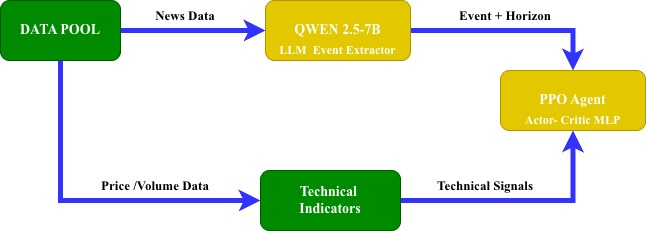
\includegraphics[width=\textwidth,height=0.26\textheight,keepaspectratio]{figs/techincal.jpg}
%   \caption{Architecture of the proposed system.}
%   \label{fig:architecture}
% \end{figure*}
% \clearpage


% Main text — add \section{Title} here when you start the next chapter (do not use \section{} with empty braces: it prints a stray number like ``3.'').
% Numbered list
% Use the style of numbering in square brackets.
% If nothing is used, default style will be taken.
%\begin{enumerate}[a)]
%\item 
%\item 
%\item 
%\end{enumerate}  

% Unnumbered list
%\begin{itemize}
%\item 
%\item 
%\item 
%\end{itemize}  

% Description list
%\begin{description}
%\item[]
%\item[] 
%\item[] 
%\end{description}  

\clearpage %%Remove this from your manuscript



% Uncomment and use as the case may be
%\begin{theorem} 
%\end{theorem}

% Uncomment and use as the case may be
%\begin{lemma} 
%\end{lemma}

%% The Appendices part is started with the command \appendix;
%% appendix sections are then done as normal sections
%% \appendix

% To print the credit authorship contribution details
\printcredits

%% Loading bibliography style file
%\bibliographystyle{model1-num-names}
\bibliographystyle{cas-model2-names}

% Loading bibliography database
\bibliography{cas-refs}

% Biography
%\bio{}
% Here goes the biography details.
%\endbio

%\bio{pic1}
% Here goes the biography details.
%\endbio

\end{document}

